\documentclass[10pt,xcolor={svgnames}]{beamer}
%\usefonttheme[onlymath]{serif}
%%%%% Colors
\usetheme{Dresden}%\usetheme{Madrid}
\colorlet{beamer@blendedblue}{green!55!black}
%%%%%

%%%%% Other 
\beamertemplatenavigationsymbolsempty
\addtobeamertemplate{navigation symbols}{}{%
    \usebeamerfont{footline}%
    \usebeamercolor[fg]{footline}%
    \hspace{1em}%
    \insertframenumber/\inserttotalframenumber
}
\usepackage{hyperref, url}
%\usepackage[symbol]{footmisc}

\definecolor{pine_green}{HTML}{007935}
\hypersetup{colorlinks,breaklinks,linkcolor=white,urlcolor=orange,citecolor=black}
\renewcommand\thefootnote{\textcolor{pine_green}{\arabic{footnote}}}
\setbeamercolor{alerted text}{fg=pine_green}

\renewcommand{\i}{\mathnormal{I}}

\usepackage{cancel}
\usepackage{ulem}
\usepackage{multirow}
\usepackage{mathtools}
\usepackage{makecell}
\usepackage{multicol}
\usepackage{tikz}
\newcommand{\tr}[1]{\textcolor{red}{#1}}
\DeclarePairedDelimiter{\abs}{\lvert}{\rvert}
\renewcommand{\epsilon}{\varepsilon}
\setbeamertemplate{itemize subitem}{\textbullet}
\setbeamertemplate{itemize subsubitem}{$\circ$}

%https://tex.stackexchange.com/questions/289542/auto-resizing-parenthesis-in-math-formulas
% \usepackage{amsmath} for testing
\newcommand*\autoop{\left(}
\newcommand*\autocp{\right)}
\newcommand*\autoob{\left[}
\newcommand*\autocb{\right]}
\AtBeginDocument {%
   \mathcode`( 32768
   \mathcode`) 32768
   \mathcode`[ 32768
   \mathcode`] 32768
   \begingroup
       \lccode`\~`(
       \lowercase{%
   \endgroup
       \let~\autoop
   }\begingroup
       \lccode`\~`)
       \lowercase{%
   \endgroup
       \let~\autocp
   }\begingroup
       \lccode`\~`[
       \lowercase{%
   \endgroup
       \let~\autoob
   }\begingroup
       \lccode`\~`]
       \lowercase{%
   \endgroup
       \let~\autocb
   }}

\delimiterfactor 1001

\makeatletter
% for amsmath "compatibility" (not sophisticated)
% \usepackage{amsmath}
\AtBeginDocument {%
          \def\resetMathstrut@{%
           \setbox\z@\hbox{\the\textfont\symoperators\char40}%
           \ht\Mathstrutbox@\ht\z@ \dp\Mathstrutbox@\dp\z@}%
}%
\makeatother
%%%%%

%%%%% Greying out/invisible Slides
%\setbeamercovered{invisible}
%\setbeamercovered{%
%  again covered={\opaqueness<1->{15}}}
  
%%%%%







%%%%% Footnotes and captions
%\usepackage[utf8]{inputenc}
\usepackage{caption}
\usepackage{comment}
\setbeamerfont{footnote}{size=\tiny}
\setbeamerfont{caption}{size=\small}
%\setbeamerfont{normal text}{size=\small}
\setbeamerfont{itemize/enumerate body}{size=\small}
\setbeamerfont{itemize/enumerate subbody}{size=\footnotesize}
%%%%%


%%%%
\usepackage{booktabs}
\usepackage{multirow,bigstrut}
\usepackage{tabu}

%%%%



%Information to be included in the title page:
\title[Connor Wiegand]{Intro to Economic Analysis: Microeconomics}
\subtitle{EC 201 - Day 19 Slides}
\author[EC 201]{Connor Wiegand}
\institute[]{Department of Economics - University of Oregon}
\date{29 November 2021}


\begin{document}

\frame{\titlepage}

\section*{Intro to Monopoly}

\begin{frame}{Logistics}
    \begin{itemize}
        \item Homework 7 due \underline{tonight} (Nov 29) at 11:59pm
        \item Homework 8 due \underline{next} Monday (Monday of finals week, Dec 6th at 11:59pm)
        \item Comprehensive final exam on \underline{December 9th} at 2:45pm -- the exam will last for 2 hours
    \end{itemize}
\end{frame}

\begin{frame}{How does a Monopolist Differ from a PC Producer?}
    \begin{itemize}%[<+->]
        \item One firm, rather than a lot of identical firms
        \begin{itemize}
            \item In class, we may use examples of oligopolies or duopolies, because true monopolies are much scarcer
            \item There are some technical differences between oligopoly and monopoly, but we will just pretend these firms are monopolies
        \end{itemize}
        \item Market power, less competition  
        \item Highly specialized products
        \item Price no longer falls from the sky
        \begin{itemize}
            \item I.e., now we have a choice of price as well as quantity
        \end{itemize}
        \item High barriers to entry
    \end{itemize}
\end{frame}

\begin{frame}{Why do Monopolies Exist}
    \begin{itemize}%[<+->]
        \item The primary reason why monopolies arise is due to high barriers of entry (examples?)
        \item These barriers of entry come in three primary forms
        \begin{itemize}
            \item Property rights
            \begin{itemize}
                \item Ex: Owning a mine, having control over a river, etc. 
            \end{itemize}
            \item Government regulation
            \begin{itemize}
                \item Ex: Intellectual property via copyrights and patents
                \item Since property is regulated by the government, there can often be overlap between this point and the previous one
                \item Ex: Coca-cola contains the sole right to legally import the coca-leaf, but this right is controlled by the government
            \end{itemize}
            \item Complex or high-fixed cost production process
            \begin{itemize}
                \item Ex: electricity grid or water distribution in a city
                \item These monopolies are often called \textit{natural monopolies}
            \end{itemize}
        \end{itemize}
        \item In my opinion, property rights usually takes the form of the other two
    \end{itemize}
\end{frame}

\begin{frame}{Natural Monopoly}
    \begin{itemize}%[<+->]
        \item The ATC curve for a monopoly might typically look like this
        \begin{figure}
            \centering
            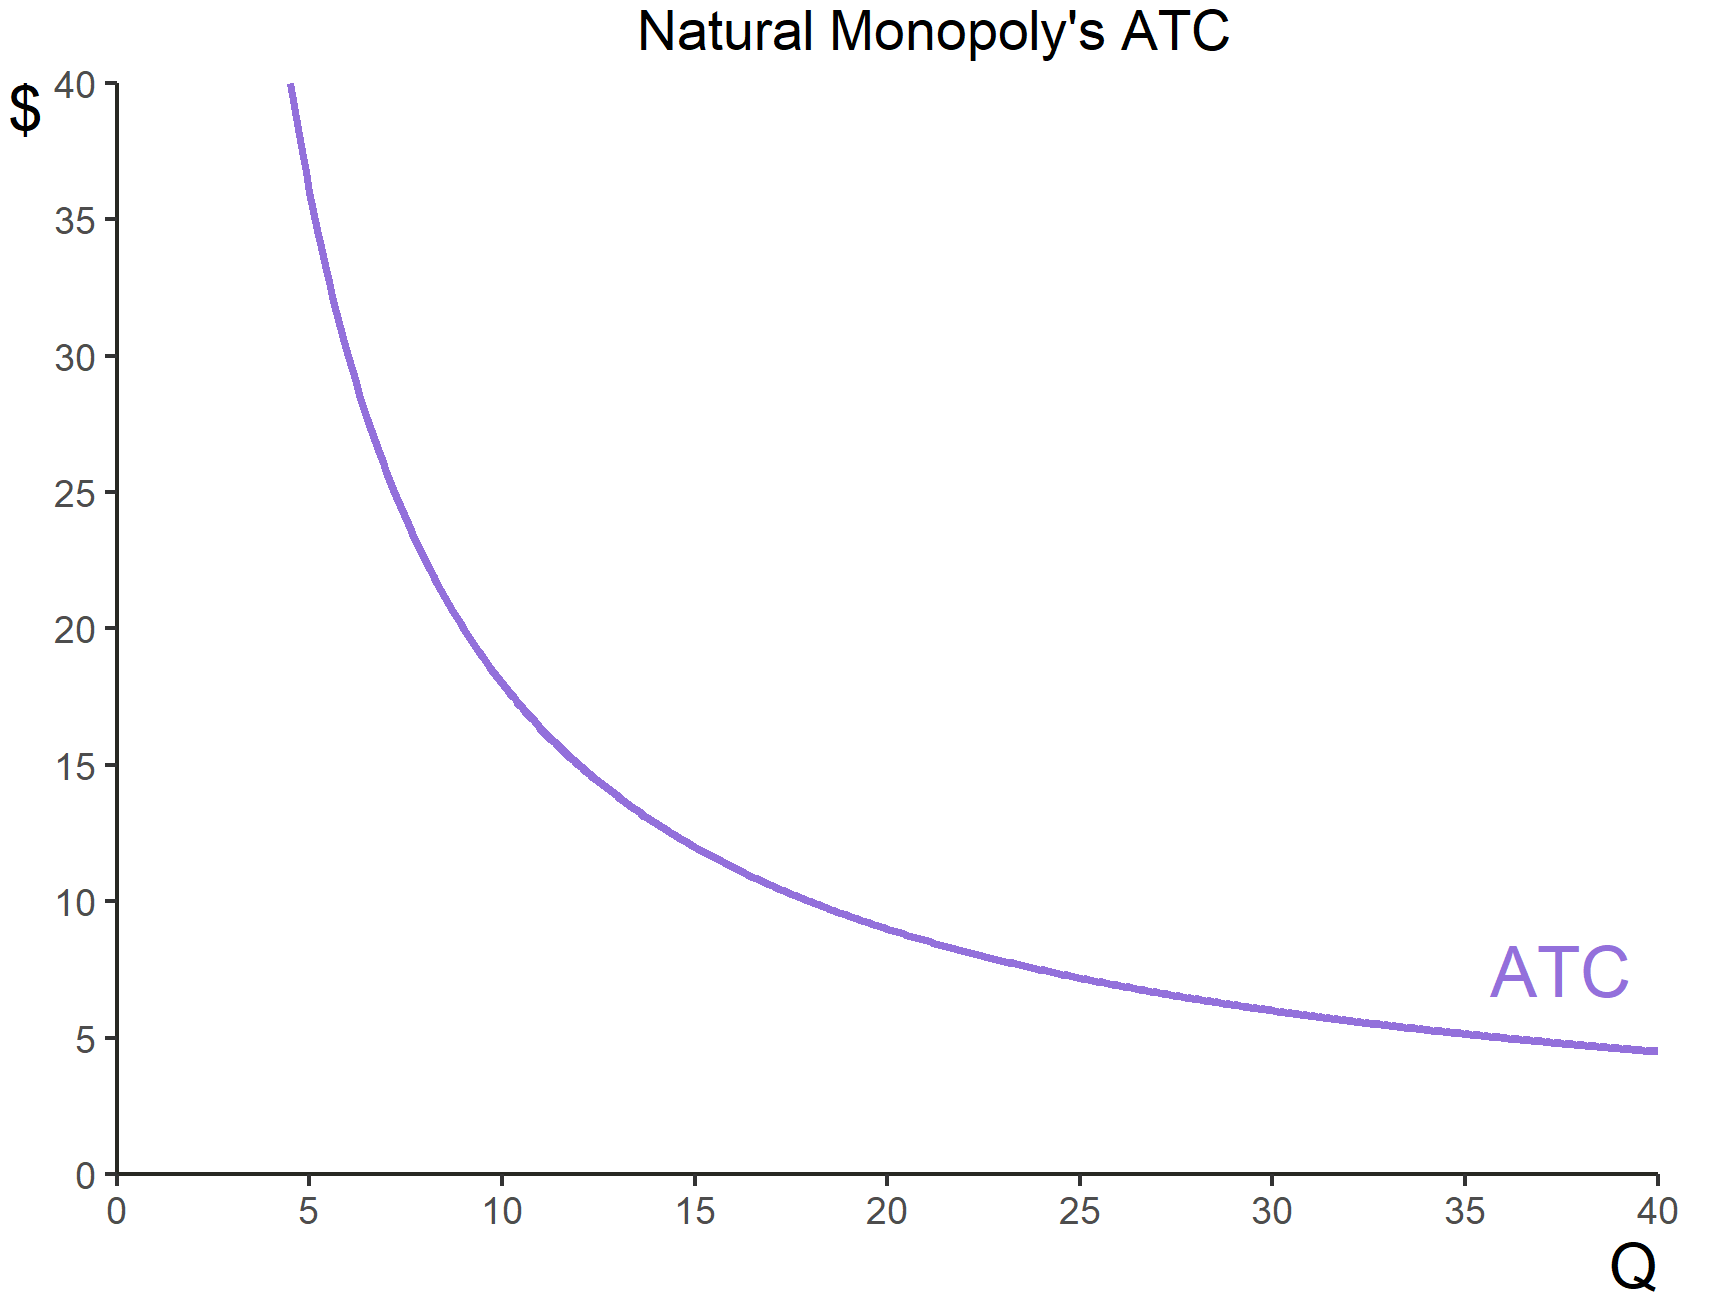
\includegraphics[width=7.5cm]{nat monop atc.png}
        \end{figure}
        \item Eventually, we might expect this curve to go back up, for very high levels of $Q$
    \end{itemize}
\end{frame}

\begin{frame}{Natural Monopoly}
        \begin{figure}
            \centering
            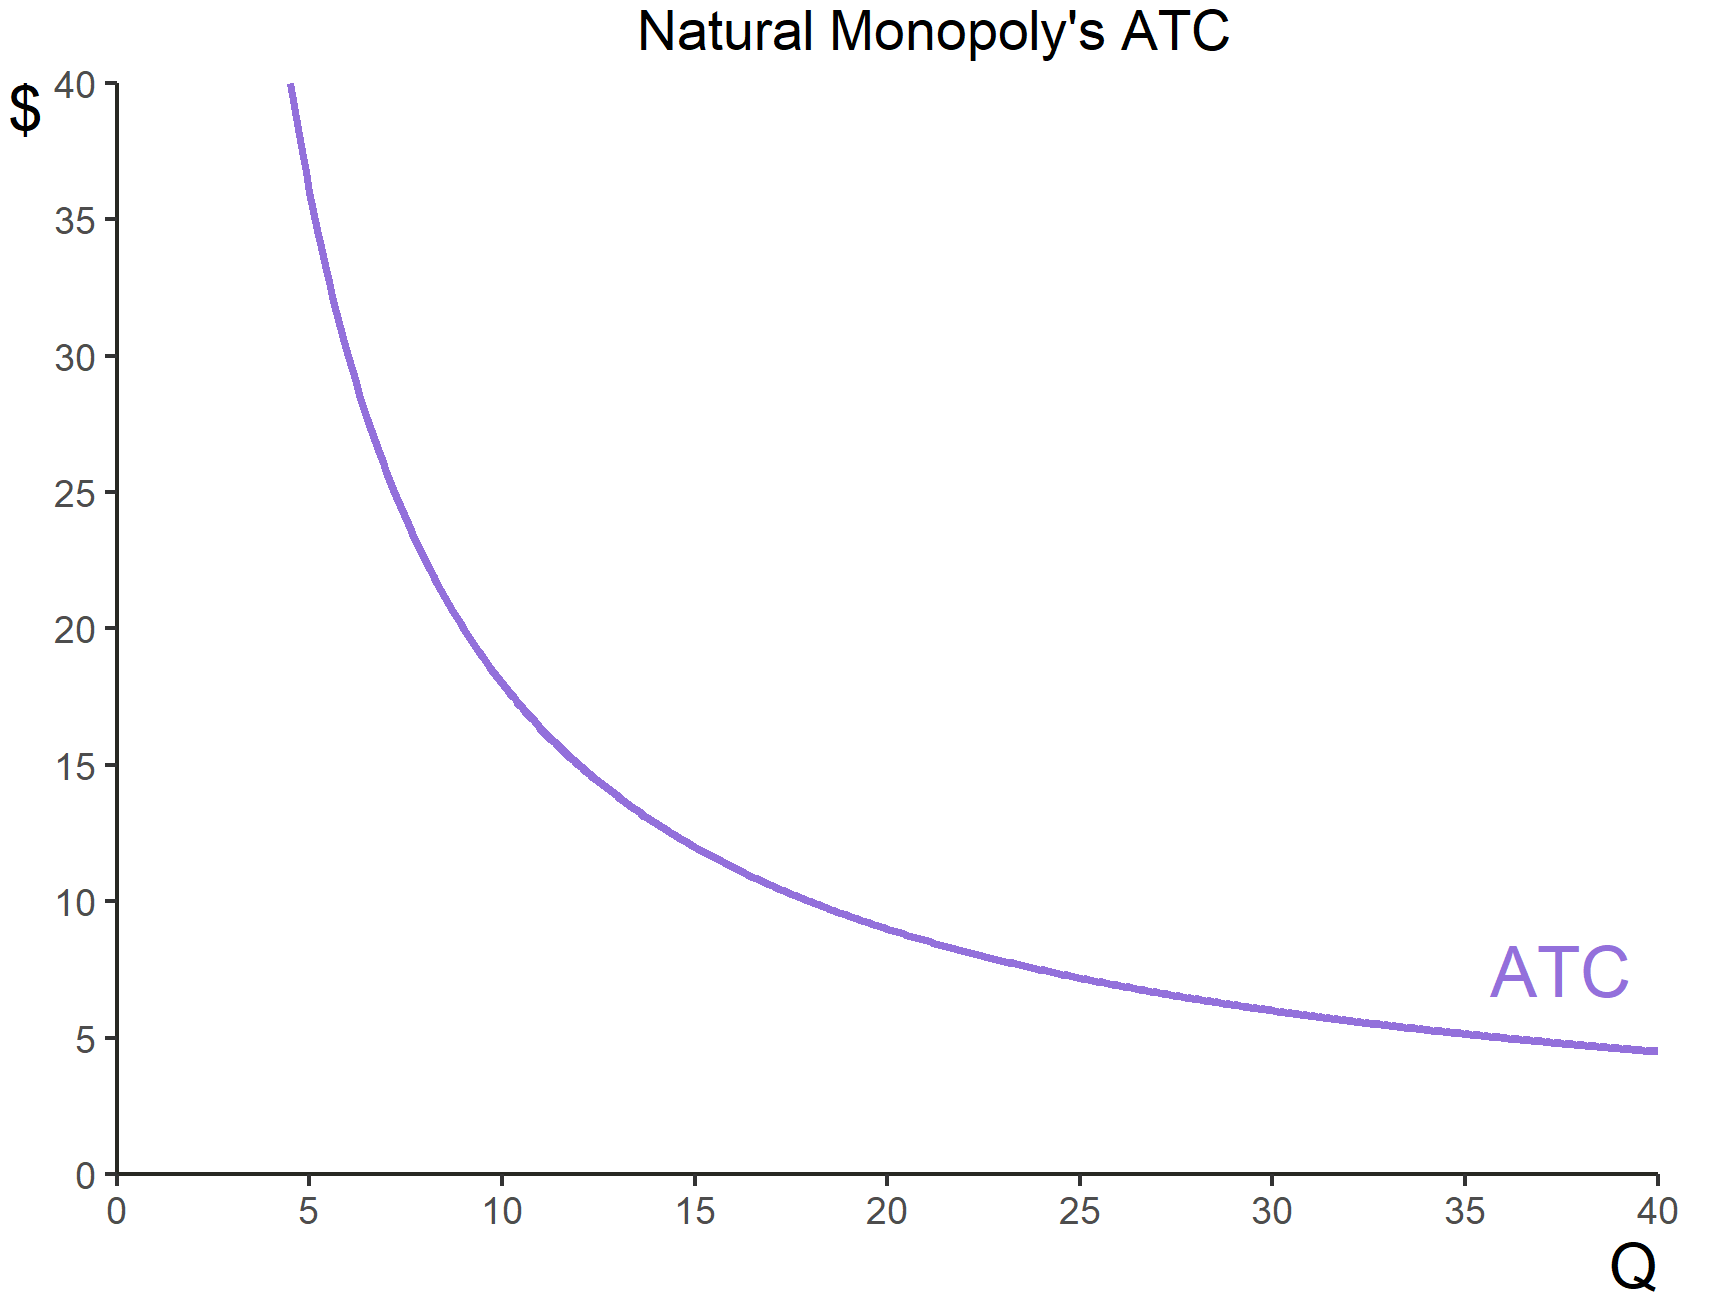
\includegraphics[width=6cm]{nat monop atc.png}
        \end{figure}
    \begin{itemize}%[<+->]
        \item Usually, this is just cause by extremely high fixed costs, and smaller/declining/more constant variable costs
        \item While most monopolies are worried about maintaining market power and need government assistance to do so, natural monopolies know that that are naturally high costs to entry and production at a small scale
    \end{itemize}
\end{frame}

\section*{Production Under a Monopoly}
\begin{frame}{}
    \begin{itemize}%[<+->]
        \item 
    \end{itemize}
\end{frame}

\end{document}